%% This is an example first chapter.  You should put chapter/appendix that you
%% write into a separate file, and add a line \include{yourfilename} to
%% main.tex, where `yourfilename.tex' is the name of the chapter/appendix file.
%% You can process specific files by typing their names in at the 
%% \files=
%% prompt when you run the file main.tex through LaTeX.
\chapter{Overview and Motivation}
\section{Introduction, Jet Definition, What a jet cross section is and why it's important}
Immediately after a quark or gluon, i.e. a "parton", is produdeced, it fragments and hadronized into energetic hadrons \footnote{almost 85\% of the constituents of jets are charged hadrons, such as $\pi^{+}, \pi^{-}, \pi^{0}, K^{+}, K^{-}, K_{L}^{0}$ and photons $\gamma$. }. The collimated spray of hadrons is called a jet. Jets are produced in abundance in hadron colliders and jet production is the dominant high transverse momentum ($p_T$) process at the LHC, and studying it gives us the best chance of understanding the physics of their original partons. The interested reader should read reviews on jets, such as \cite{towards_jetography}.

In the CMS experiment, jets are reconstructed from energy deposits (trigger primitives) of final stable particles (the jet constituents with lifetime $c \tau > 1 \ cm$) in the calorimeter towers. These energy deposits are then used as input to a clustering algorithm in which a seed particle $i$ sets some initial direction, and one sums the momenta of all particles $j$ within a circle (“cone”) of radius $R$ around $i$ in azimuthal angle $\phi$ and rapidity $y$ (or pseudorapidity $\eta$)  i.e. taking all particles $j$ such that $\Delta R_{i j}^{2}=\left(y_{i}-y_{j}\right)^{2}+\left(\phi_{i}-\phi_{j}\right)^{2}<R^{2}$. 
% \footnote{In the LHC, the beam direction is assumed to be in the $z$ axis, and the $x-y$ plane is perpendicular to the beam. $\theta$ is the angle between the particle momentum diirection and the $z$ direction. A particle with energy $E$ and momentum along the beam direction $p_z$ has rapidity $y \equiv \frac{1}{2} \ln \frac{E+p_{x}}{E-p_{x}}$ and pseudorapidity $\eta \equiv-\ln \tan \theta / 2$. Massless particles have $y=\eta$, and differences in rapidity are invariant under longitudinal (along the beam direction) boosts. }

\begin{figure}
    \centering
    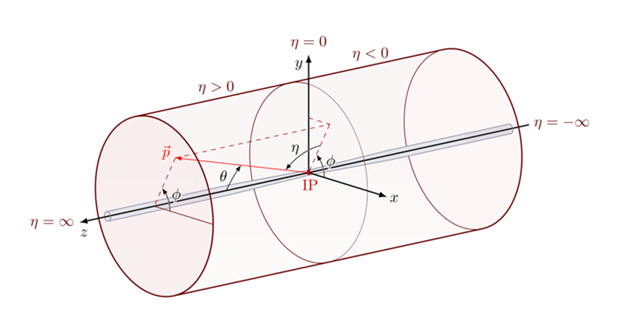
\includegraphics[width=12.5cm,height=6cm]{templates/CMS_coordinates.png}
    \caption{In the LHC, the beam direction is assumed to be in the $z$ axis, and the $x-y$ plane is perpendicular to the beam. $\theta$ is the angle between the particle momentum diirection and the $z$ direction. A particle with energy $E$ and momentum along the beam direction $p_z$ has rapidity $y \equiv \frac{1}{2} \ln \frac{E+p_{x}}{E-p_{x}}$ and pseudorapidity $\eta \equiv-\ln \tan \theta / 2$. Massless particles have $y=\eta$, and differences in rapidity are invariant under longitudinal (along the beam direction) boosts.}
    \label{CMS_coordinates}
\end{figure}
The most efficient and widely-used clustering algorithm is the anti-kt algorithm, usually implemented in the FastJet package.


After jets have been reconstructed, studying them can offer treasure trove of information about fundamental physics. One of the best best studied things in the LHC related to jets is the inclusive jet spectrum, which is related to the momentum transfer $2 \rightarrow 2$ scttering of partons inside the proton. In this process, the energy of a the jet is closely related to that of the hard scattering of partons inside the protons, therefore the inclusive jet spectrum quantifies the distributions of partons inside the proton.




Measurements of the inclusive jet and dijet cross sections are classical particle physics measurements and are benchmarks of the standard model at particle colliders. Such measurements have been measuren in $e^+ e^-, ep, pp,$ and $p \bar{p}$ colliders. They have been used to test the predictions of perturbative QCD, have given precise measurements of the strong coupling constant $\alpha_S$, have been used to obtain information about the structure of the photon and neutron by constraining parton distribution functions (PDFs) of theproton (as well as differentiate between PDF sets), and  have been used to look for possible deviations from the standard model.  








\section{What is a cross section and what are PDFs?}
The total scattering cross section is computed by convoluting the parton distibution function for each incoming parton from each proton with the corresponding partonic level cross section.

Hence, in the language of QCD, the short-distance (high energy) part of the process can be computed from perturbation theory, and long-distance (low energy) part of the process is driven by the non-perturbative nature of QCD at low-energy scales. Collinear factorization theorem allows us to separate the perturbative (calculable) hard part of the process from the non-pertubative one, which can be described in terms of parton distribution (or fragmentation) functions. The total cross section of inelastic proton-proton scattering to produce a final state $n$ can be calculated with the formula
\begin{equation}
    \sigma = \sum_{a, b} \underbrace{\int_{0}^{1} d x_{a} d x_{b} f_{a/A}\left(x_{a}, \mu_{F}\right) f_{b/B}\left(x_{b}, \mu_{F}\right)}_{\text{long-distance, non-perturbative PDF part}} \times \underbrace{\int d \Phi_{n}  \frac{1}{2 \hat{s}}\left|\mathcal{M}_{a b \rightarrow n}\right|^{2}\left(\Phi_{n} ; \mu_{F}, \mu_{R}\right)}_{\text{short-distance "hard" perturbative part}}
    \label{QCD_master}
\end{equation}
Where $f_{a/A}(x, \mu)$ denotes the parton distribution functions, which depend on the momentum fractin $x$ of a parton $a$ with respect to its parent hadron $A$, and on an arbitrary energy scale called the factorization scale $\mu_F$. $d \Phi_{n}$ is the differential phase space element over $n$ final-state particles,
\begin{equation}
    d \Phi_{n}=\prod_{i=1}^{n} \frac{d^{3} p_{i}}{(2 \pi)^{3} 2 E_{i}}(2 \pi)^{4} \delta^{(4)}\left(p_{a}+p_{b}-\sum_{i=1}^{n} p_{i}\right)
\end{equation}
Where $p_a$ and $p_b$ are the initial state momenta. 
The convolution of the squared matrix element $\left|\mathcal{M}_{a b \rightarrow n}\right|^{2}$ 
, averaged over initial-state spin and colour degrees of freedom, with the
Lorentz-invariant phase space Φn and multiplied by the flux factor $ 1/(2ˆs) = 1/(2xaxbs)$
results in the calculation of the parton-level cross section $\hat{\sigma}_{ab→n}$. 

Hence we can intuitively say that the differential cross section in transverse momenta of the observed jet can be factorized in the following form \footnote{sometimes this is called the "master formula"}
\begin{equation}
\frac{d \sigma_{jet}}{d \mathcal{O}} \sim\\
\sum_{a, b} \int d x_{a} f_{a / A}\left(x_{A}, \mu\right) \int d x_{b} f_{b / B}\left(x_{B}, \mu\right) \frac{d \sigma_{partons}}{\mathcal{O}}
\label{master}
\end{equation}
Where $\sigma_{partons}=\int d \Phi_{n}  \frac{1}{2 \hat{s}}\left|\mathcal{M}_{a b \rightarrow n}\right|^{2}\left(\Phi_{n} ; \mu_{F}, \mu_{R}\right)$ can be seen from \ref{QCD_master}, and $ \mathcal{O}$ is any jet observable for example the jet $p_T$ or the rapidity $|y|$. The equation \ref{master} illustrates the principle of \emph{factorization}  i.e. that short distance and long distance processes are separable such that they can be convoluted in this manner, so that the "hard part" $\sigma_{partons}$ and "normalizations" from the PDFs are on diffrent scales.   Factorization also posits that the PDFs are universal, i.e. process-independent. 


The parton level cross sections $d \sigma_{partons}$ has an expansion in powers of $\alpha_S$
\begin{equation}
    \frac{d \sigma_{partons}}{d P_{T}} \sim \sum_{N}\left(\frac{\alpha_{s}(\mu)}{\pi}\right)^{N} H_{N}\left(x_{A}, x_{B}, P_{T} ; a, b ; \mu\right)
    \label{patron_x}
\end{equation}
Where the coefficients $H_N$ are calculable in perturbative QCD. Equation \ref{parton_x} demonstrates the principle of \emph{Asymptotic Freedom}, i.e. hard scattering is weak at short distances, and hence perturbatively calculable. At next-to-leading-order and beyond, however, the calculation will involve divergences that must be removed, and the dependence on the scale $\mu$ will appear in their place. 

% Inclusive jet cross section measurements are typically defined by the anti-$k_T$ algorithm implemented in the FASTJET package. Such an algorithm is infrared-safe and boost-invariant along the z-axis. The algorithm has proven to be the most effective in keeping the background induced from pileup (i.e. from other interactions) under contril by keeping the jets circular in the $(y, \phi)$ plane with a radius radious roughly equal to the jet size parameter $R$.















\section{Short-term and long-term plan for my thesis}
As Run 3 will start later this year, the timing of my dissertation seems apt to analyze Run 1 and
2 data, as well as be one of the first to analyze Run 3 data. Although I have worked and still
work on many different projects in ML, PDFs, HGCAL, database, prefiring, my dissertation
will in a big picture view be composed of two parts: a short-term plan, which I define as my plan up to the next year, and a long-term plan, which is defined as my plan until I graduate, estimated to be 2 or 3 years. 

For my short term plan, I am going to be a part of a team at DESY that will use the full Run 2 dataset to measure the inclusive jet cross section. I plan to go to DESY this summer to work on this project, and our team plans to publish a paper on this measuremtn next year of which I will be one of the main co-authors.

For my long term plan, which will take the bulk of the writing that is to follow, I plan to do my own inclusive jet cross section measurement using the preliminary Run 3 data, but I will be using a novel observable for which there is only a single observable per event. This is done so that we can avoid cross problematic correlations between the different channels/bins. Having measured this cross section over the full $p_T$ range, we will use that to do a EFT fit. The novelty in our EFT fit is that this time we will do a true global fit, without making any assumptions about the EFT coeffiecients. This means that we will fit all the EFT (Wilson) coefficients simultaneously resulting in a full-scale modelling of the probability distributions of the Wilson coefficients. This would give the best chance of saying something about dimension-6 operators that might set bounds on new physics, as well as searching for contact interactions. 